        \section{Old outgroup checklist}

        
        \subsection{Other families}
        
    \subsubsection{PF01388 - ARID - CL0123 (HTH)}
Although ARID (PF01388) was not found by JackHmmer, there is a structural similarity between RHH\_1 and ARID and likely to other families from the HTH clan.

\begin{itemize}
    \item CLANS
\end{itemize}
Family is rather small and separation I think separating into groups shouldn't be considered here.
\begin{figure}[H]
\begin{center}
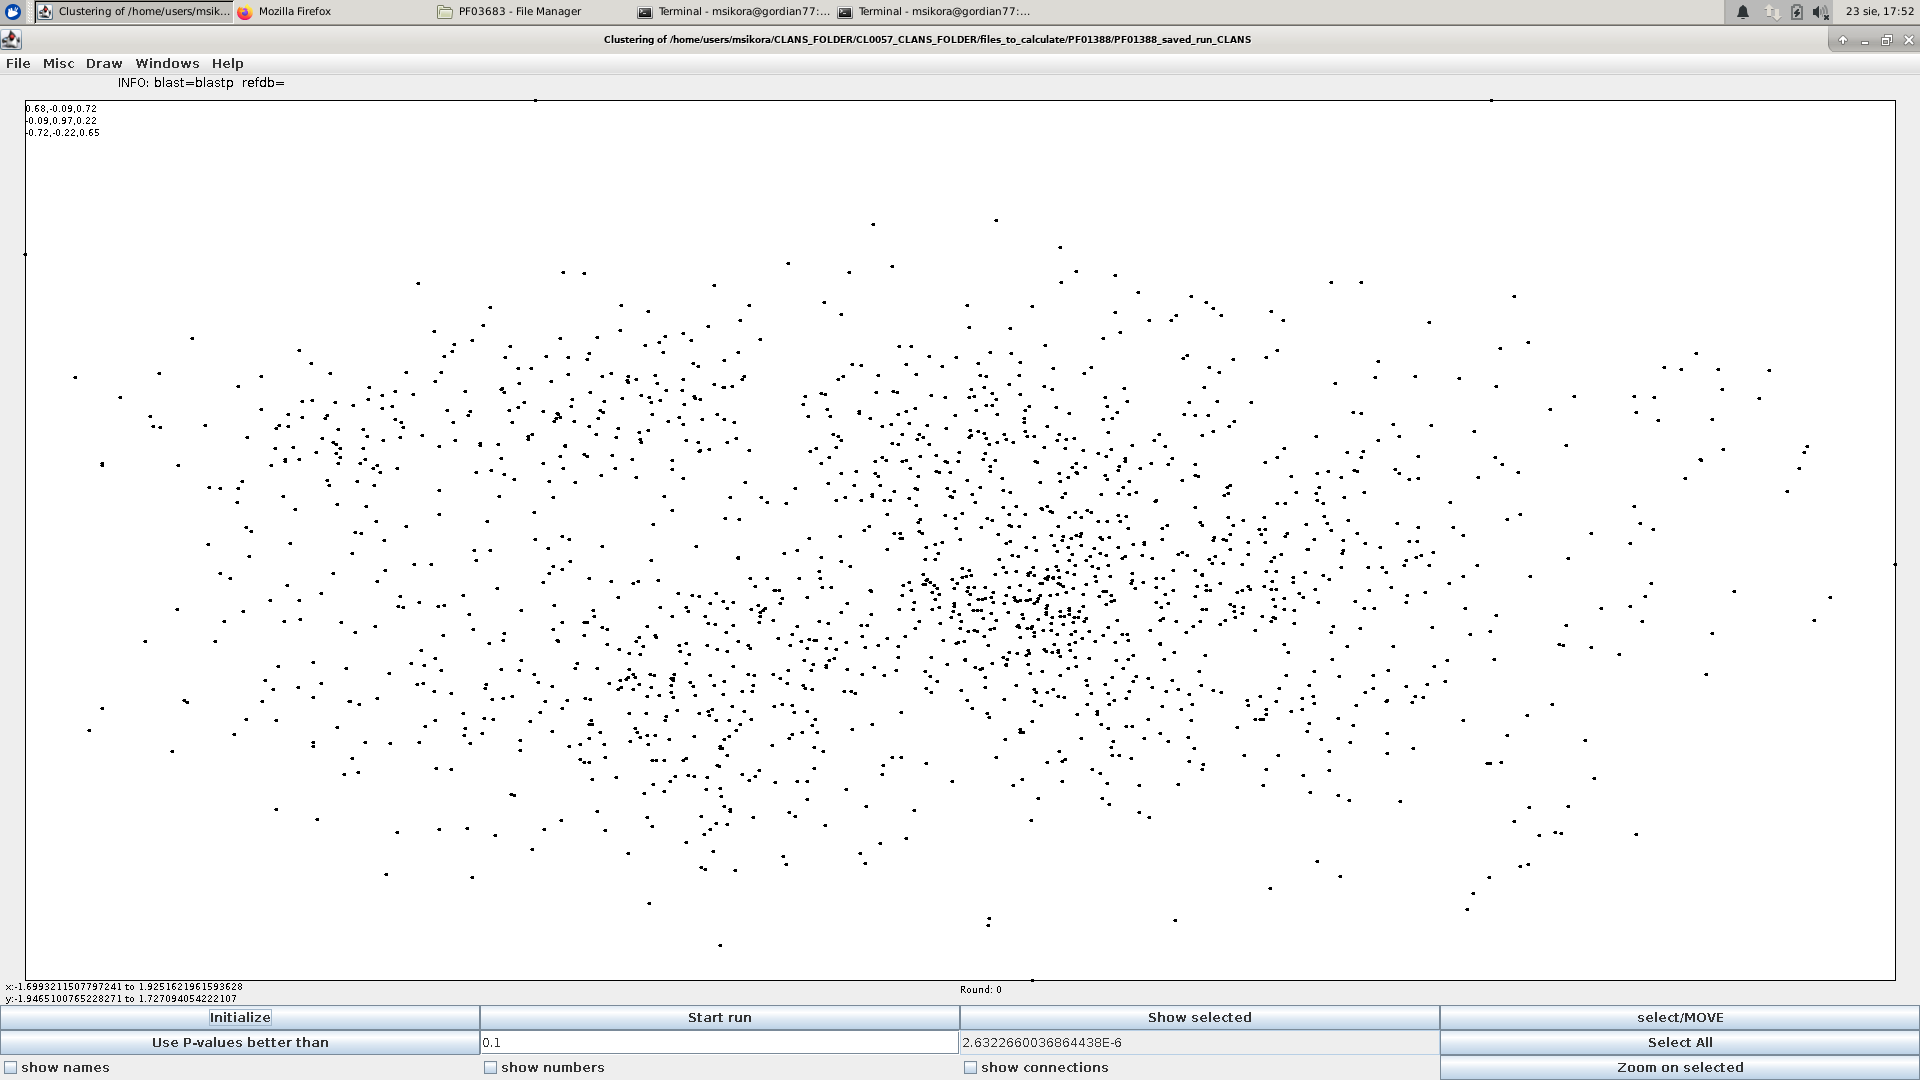
\includegraphics[width=0.5\textwidth]{PF01388_CLANS.png}
\end{center}
\end{figure}

    \subsubsection{PF13443 - HTH\_26 - CL0123 (HTH)}
PF13443, PF01381 aligned with each other, because they are from the same clan.
Although HTH fold is similar to RHH, there is no significant sequence similarity.

\begin{itemize}
    \item CLANS
\end{itemize}
Not so clear groups, however, it might be possible to separate it into 5 groups (4 smaller and 1 big).
\begin{figure}[H]
\begin{center}
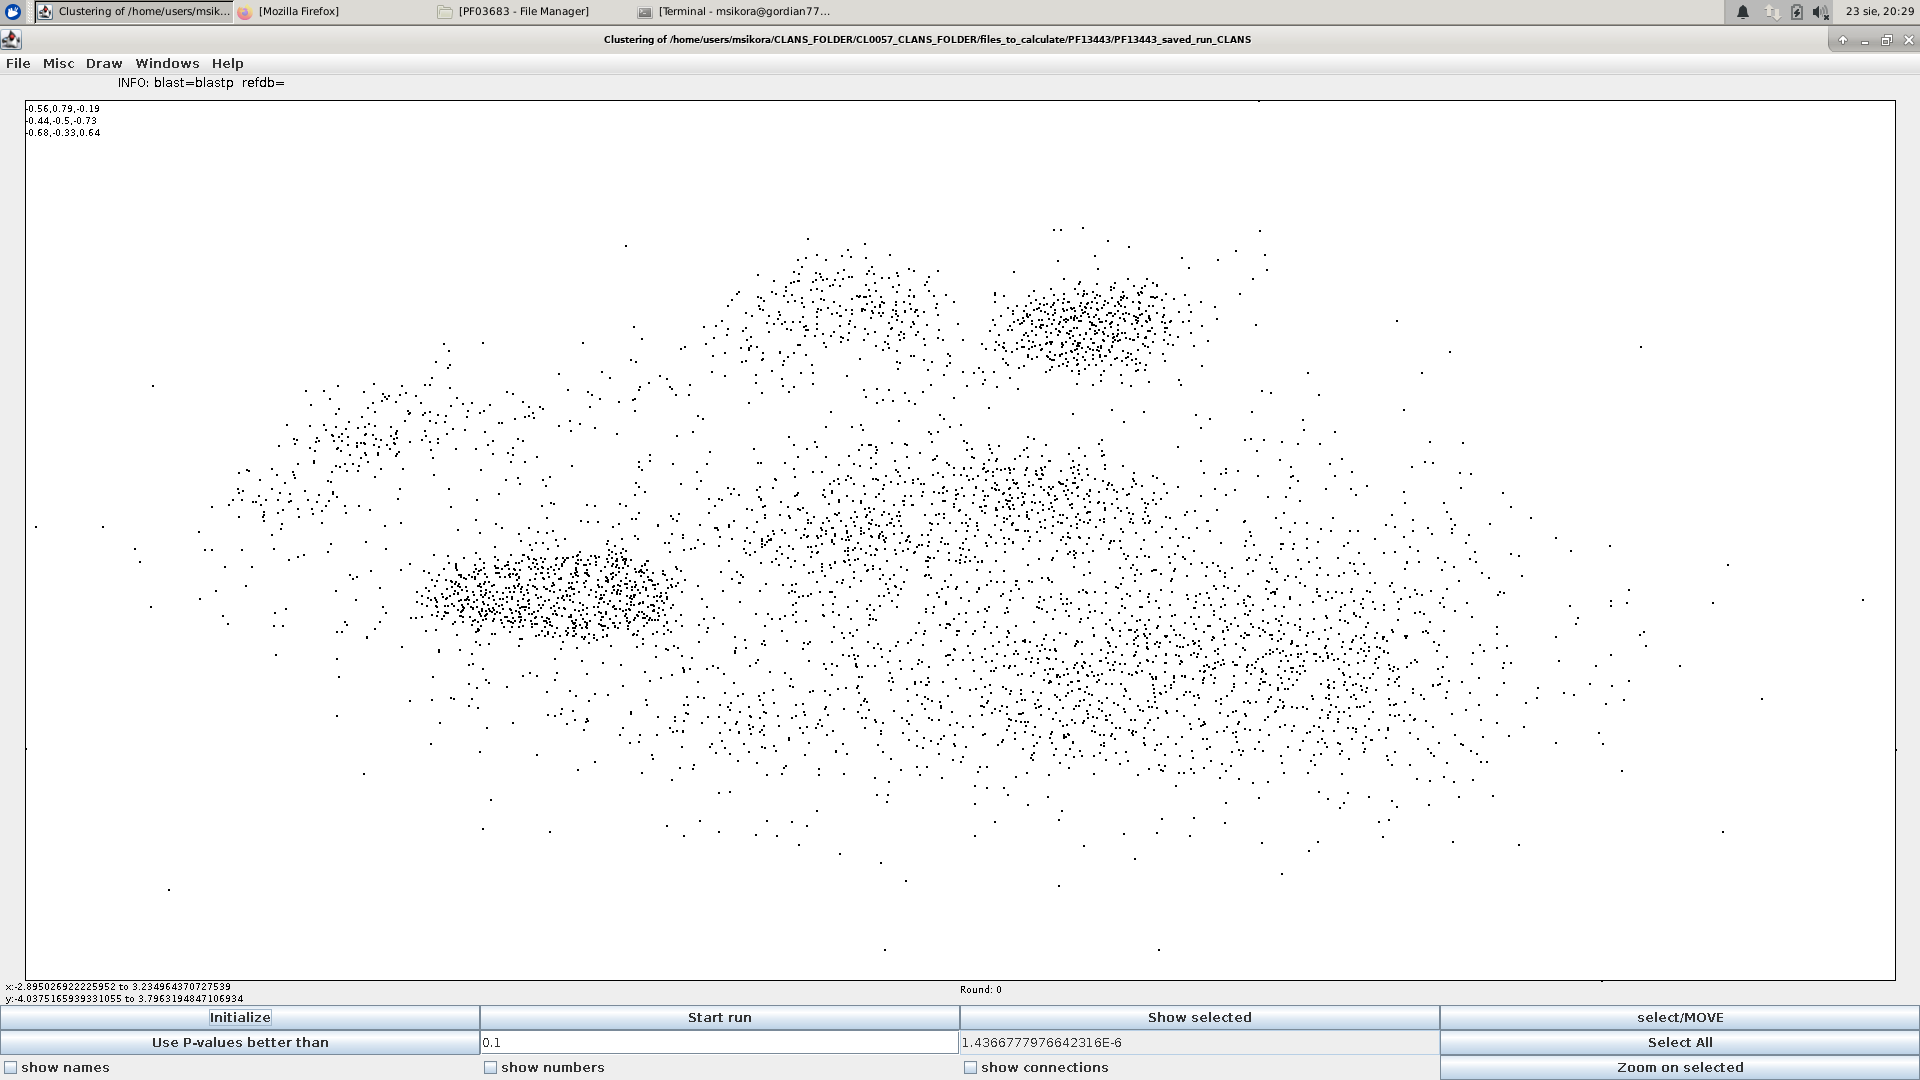
\includegraphics[width=0.5\textwidth]{PF13443_CLANS.png}
\end{center}
\end{figure}

    \subsubsection{PF01381 - HTH\_3 - CL0123 (HTH)}
PF13443, PF01381 aligned with each other, because they are from the same clan.
Although HTH fold is similar to RHH, there is no significant sequence similarity.

\begin{itemize}
    \item CLANS
\end{itemize}
Separating into 1 main group and 4 subgroups (or just 1 extra) may be considered.

\begin{figure}[H]
\begin{center}
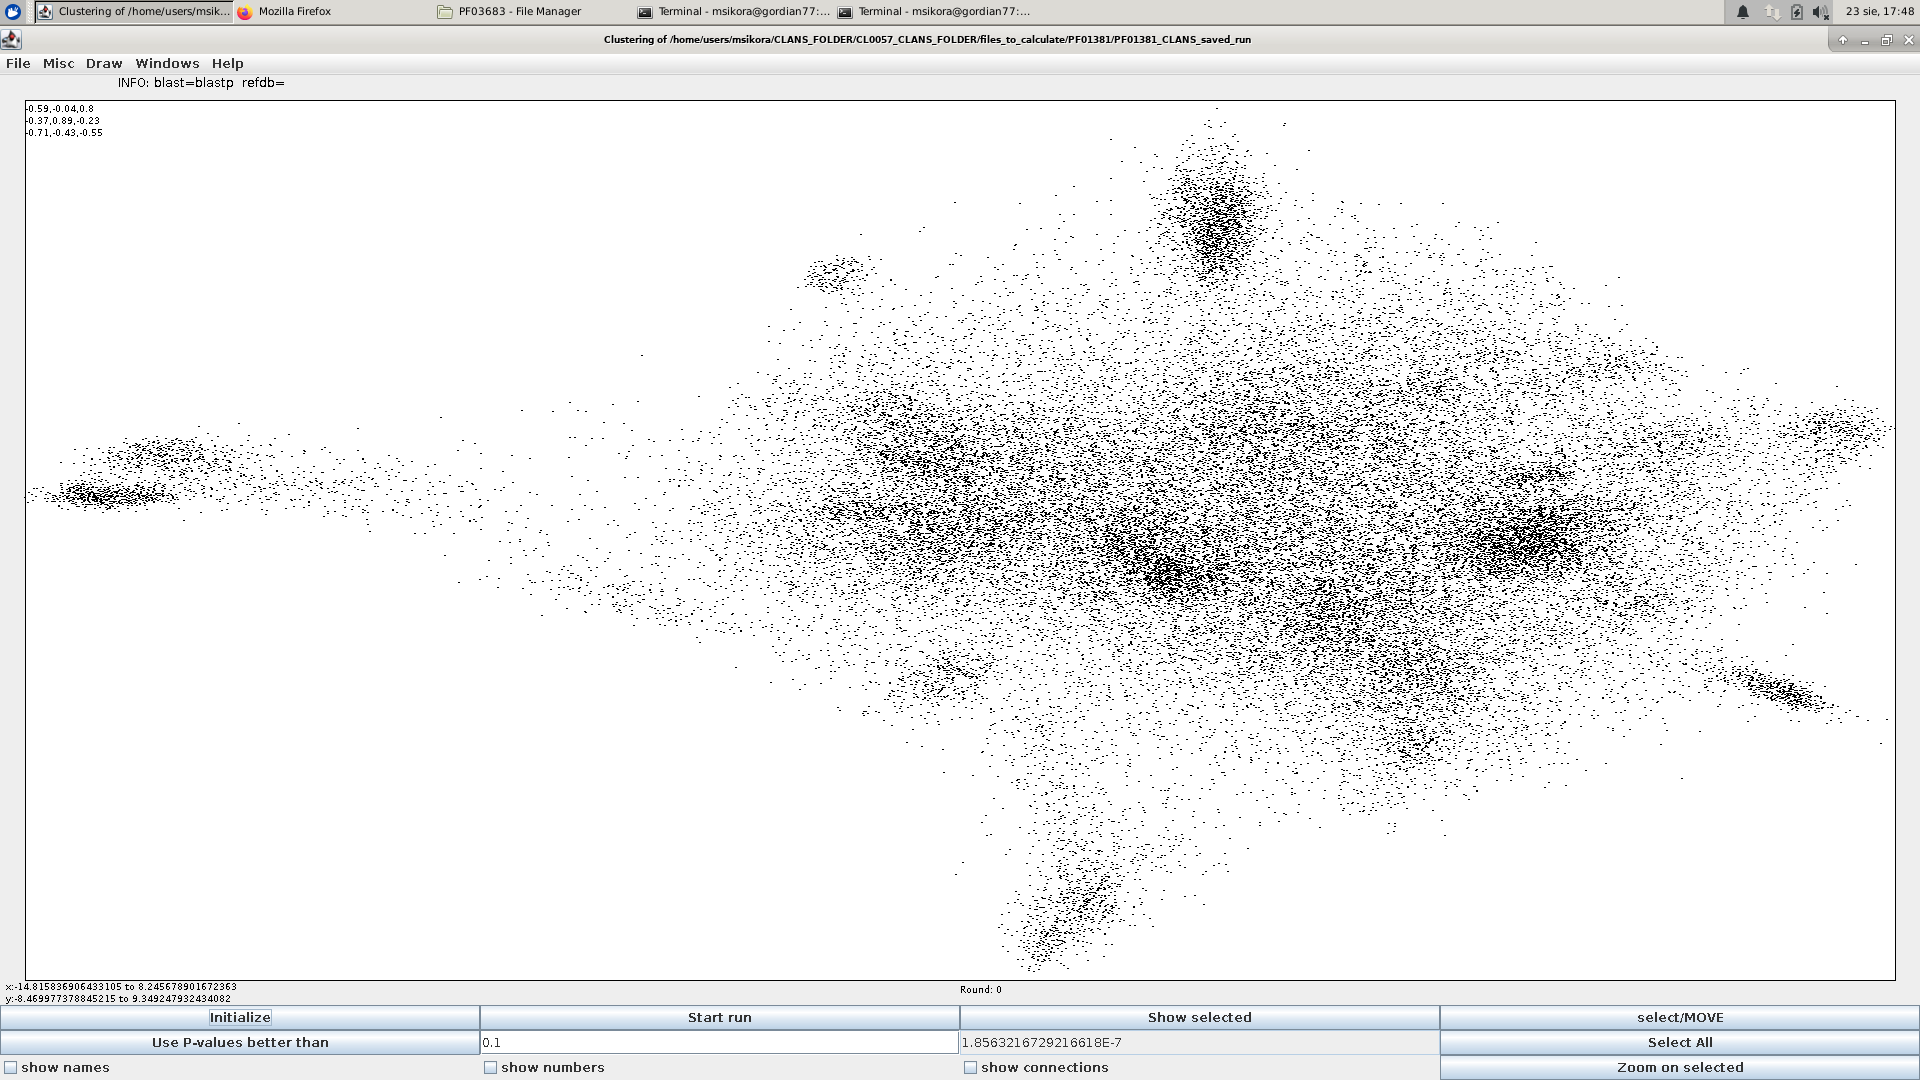
\includegraphics[width=0.5\textwidth]{PF01381_CLANS.png}
\end{center}
\end{figure}

    \subsubsection{PF03683 - UPF0175 - CL0123 (HTH)}
\begin{itemize}
    \item CLANS
\end{itemize}
I wouldn't separate this family into groups, as one group wouldn't have enough sequences.
\begin{figure}[H]
\begin{center}
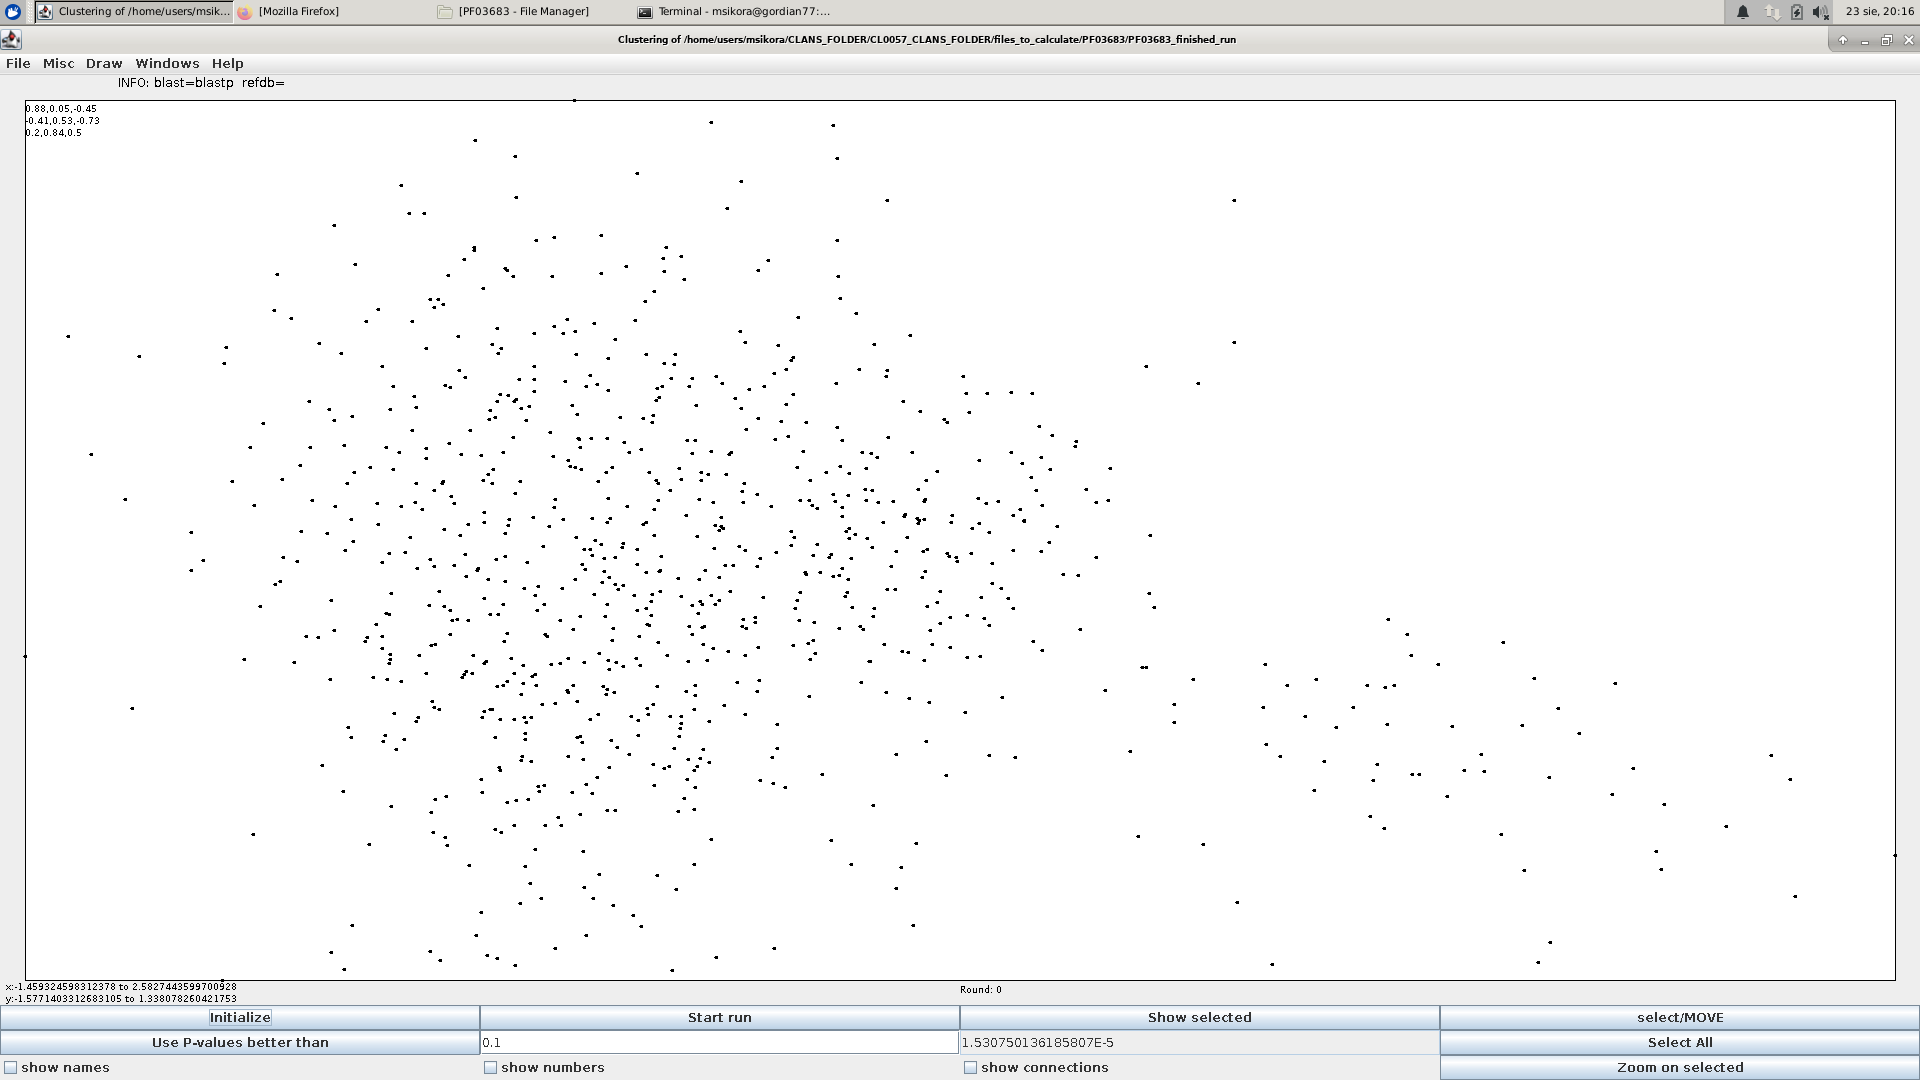
\includegraphics[width=0.5\textwidth]{PF03683_CLANS.png}
\end{center}
\end{figure}

    \subsubsection{PF17373 - DUF5395 - No clan}
Not aligned to the RHH column.
Aligned to PHD-like domain of PF15919 (1st column)
DOMAIN of PF15919 - HicB\_like antitoxin of bacterial toxin-antitoxin system!!! (Difference between Pfam and \ldots?)

\begin{itemize}
    \item CLANS
\end{itemize}
Not enough sequences for separation.
\begin{figure}[H]
\begin{center}
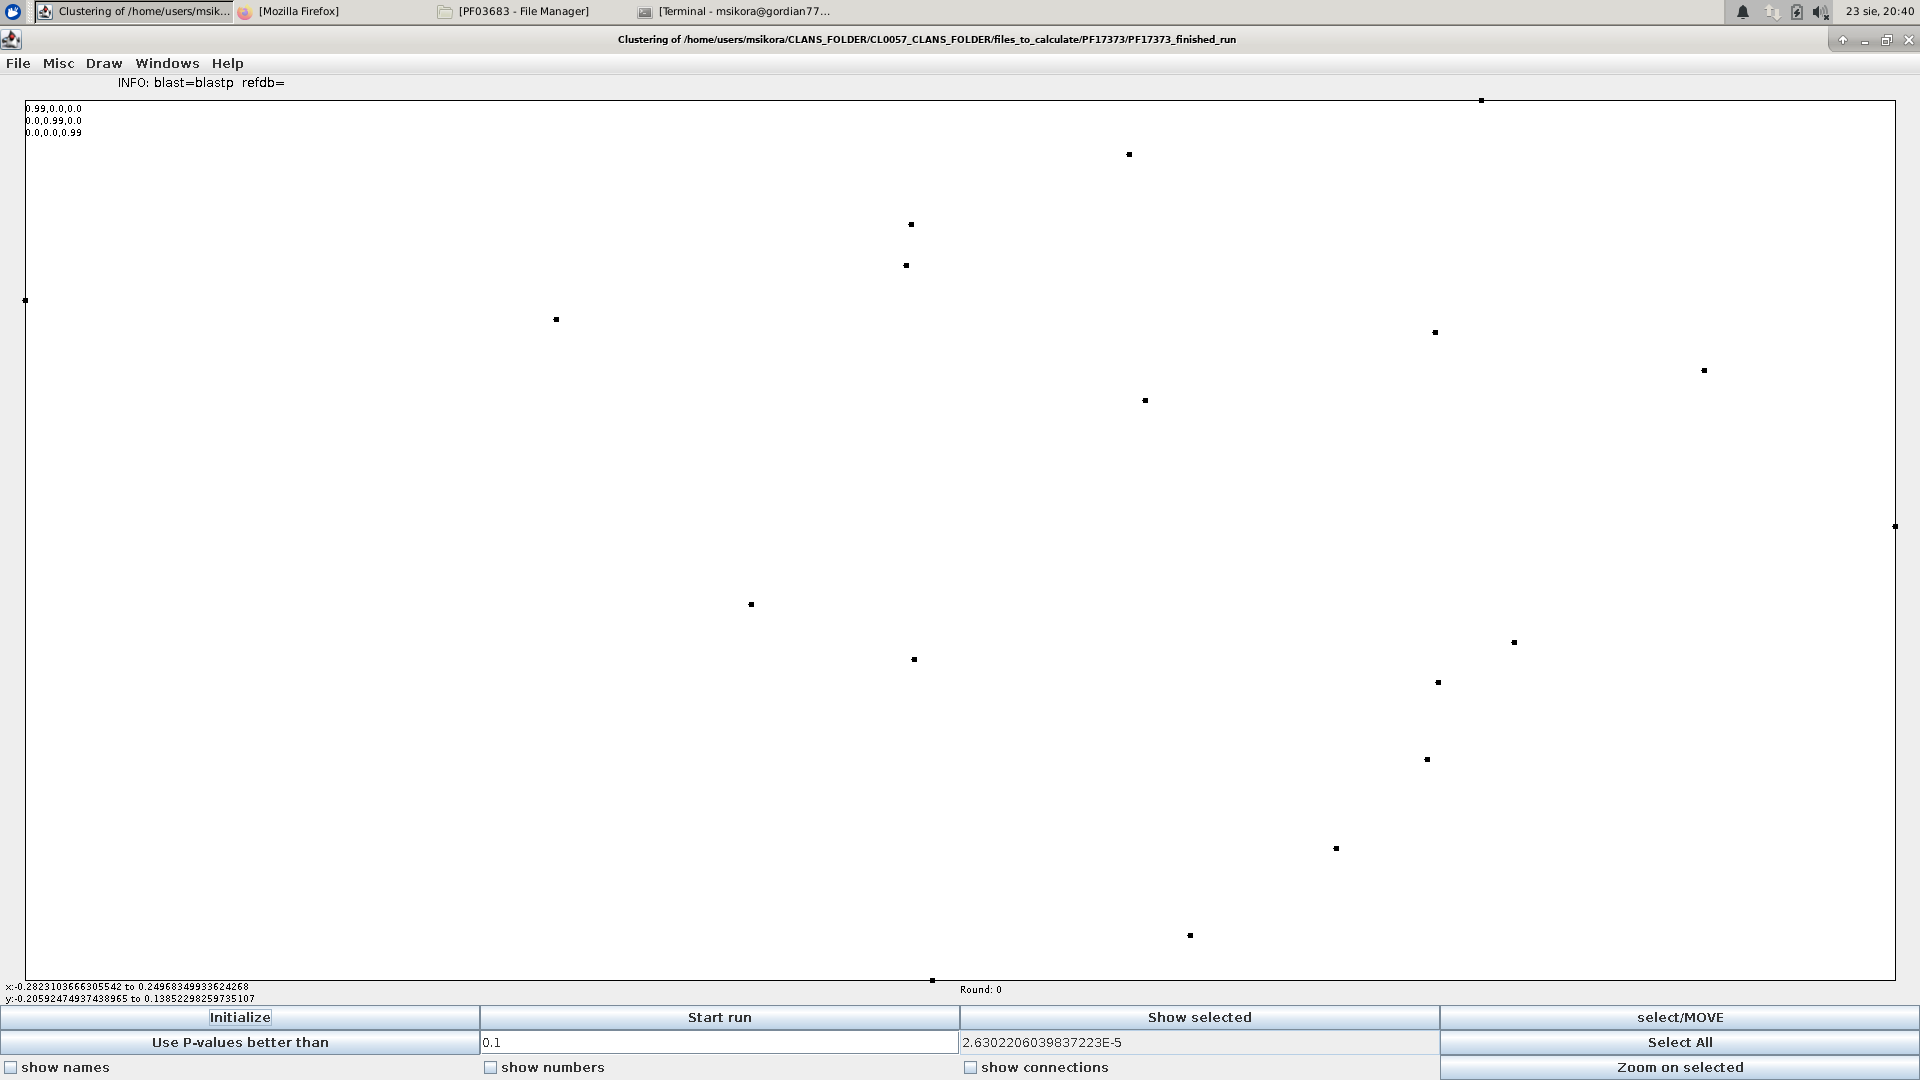
\includegraphics[width=0.5\textwidth]{PF17373_CLANS.png}
\end{center}
\end{figure}

    \subsubsection{PF12910 - PHD\_like - CL0136 (Plasmid antitox)}
PHD\_like (PF12910) - this domain appears to be the N-terminus of the RelB antitoxin of the toxin-antitoxin stability system.
Therefore it is related in function to Met\_repress.
However, HicB\_lk\_antitox (PF15919) Pfam domain has a long seq (~ 140 residues), so it contains not only the RHH motif but also another domain.
PHD\_like (PF12910) aligns with another domain of HicB\_lk\_antitox (not RHH motif), therefore it appears in this search, but it is not relevant for RHH motif.

\begin{itemize}
    \item CLANS
\end{itemize}
Separating into 2 groups may be considered, however they will have only few sequences in each.
\begin{figure}[H]
\begin{center}
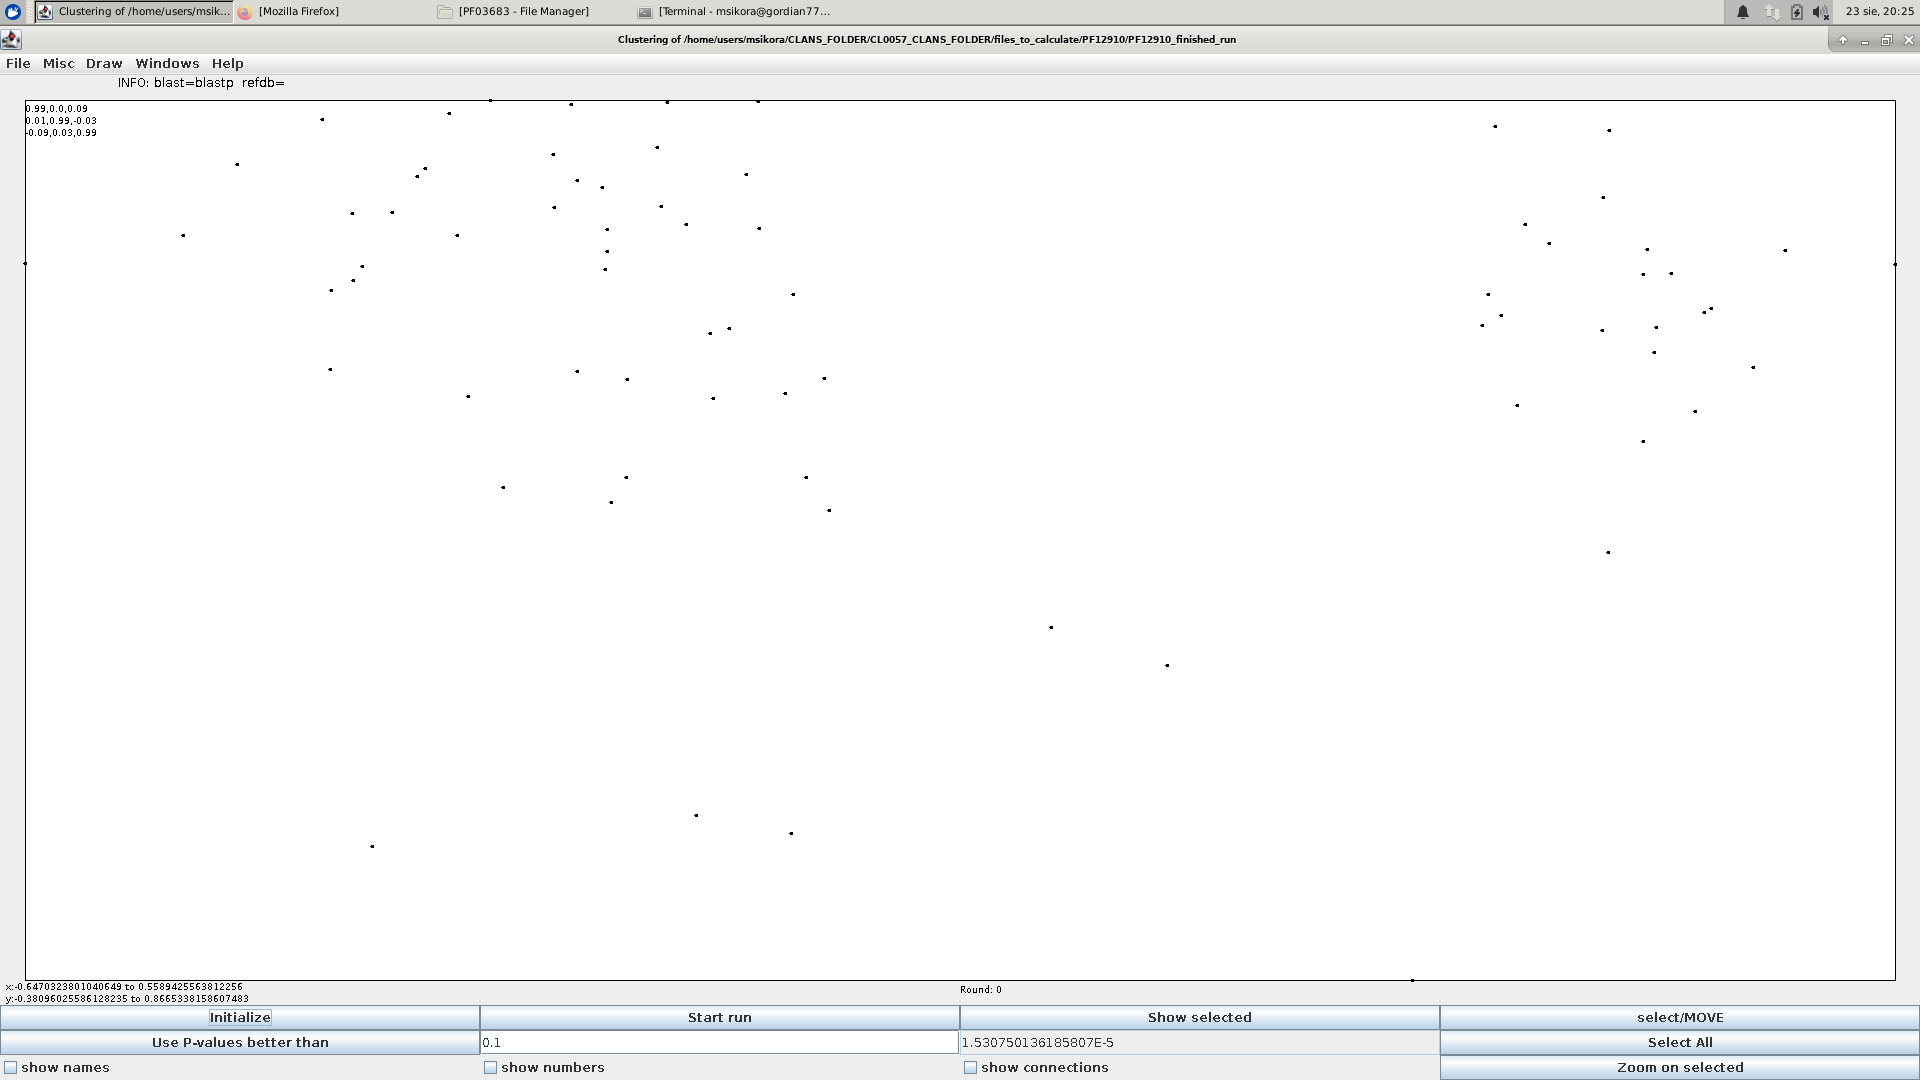
\includegraphics[width=0.5\textwidth]{PF12910_CLANS.png}
\end{center}
\end{figure}

    \subsubsection{PF05261 - Tra\_M / DNA-binding - CL0548 (IHF-likeDNA-bdg)}
Aligning with center column.
\begin{itemize}
    \item CLANS
\end{itemize}
Nothing to separate - there are only 19 sequences in the family.
\begin{figure}[H]
\begin{center}
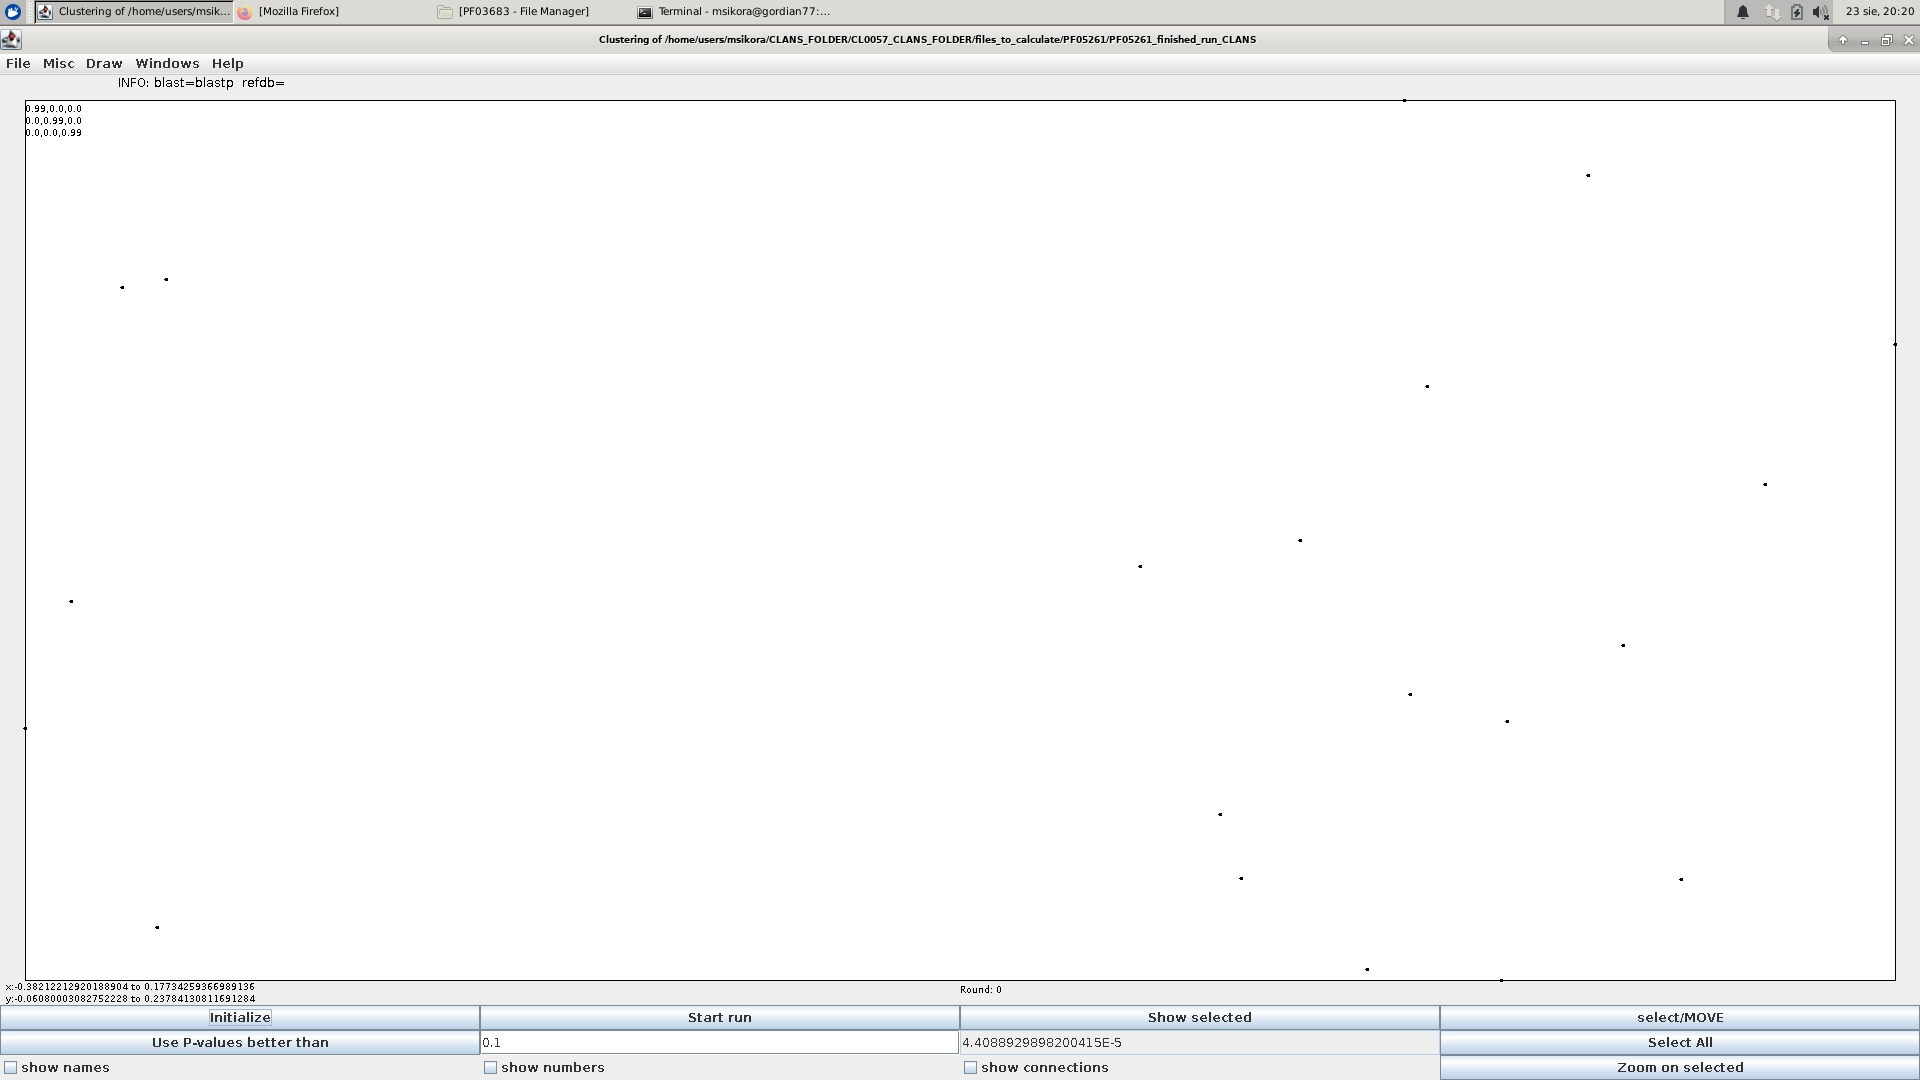
\includegraphics[width=0.5\textwidth]{PF05261_CLANS.png}
\end{center}
\end{figure}

   \subsubsection{PF01865 - PhoU\_div / DUF47 - CL0297 (PhoU)}

\begin{itemize}
    \item CLANS
\end{itemize}
Separation into 2 groups may be considered as seen below.
\begin{figure}[H]
\begin{center}
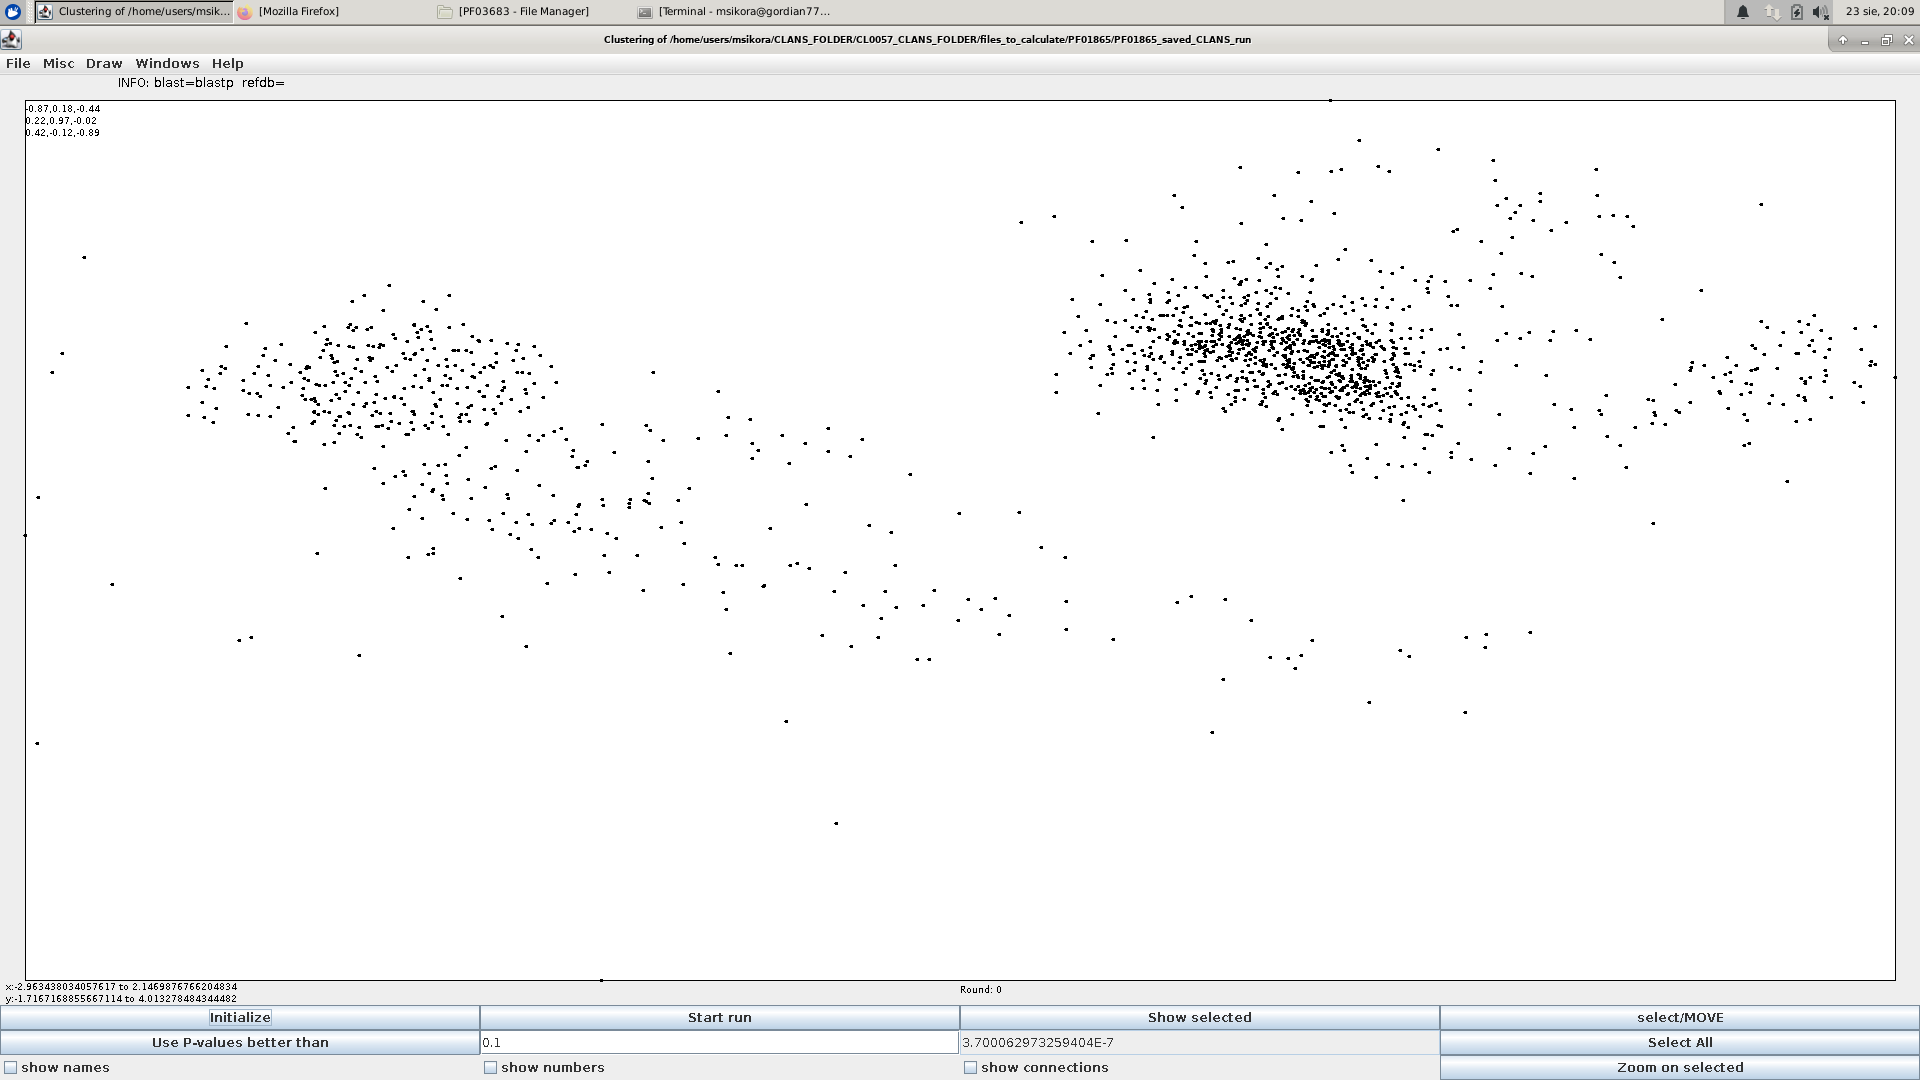
\includegraphics[width=0.5\textwidth]{PF01865_CLANS.png}
\end{center}
\end{figure}

   \subsubsection{PF00096 - Zinc finger, C2H2 type - CL0361 (C2H2-zf)}
Domains are very short (around 20 AA), and there are way too many sequences.

I was able to push the family into Ola's workflow, no results.

\begin{itemize}
    \item CLANS
\end{itemize}
Unable to finish CLANS .
First part - BLAST - finished, however, I'm unable to load sequences into second part - clustering - Out of memmory errors.


   \subsubsection{PF13517 - VCBS / Repeat domain in Vibrio, Colwellia, Bradyrhizobium and Shewanella - CL0186 (Beta propeller)}
\begin{itemize}
    \item CLANS
\end{itemize}
It might be possible to separate each ''spike'', but what about middle cloud?
I'm not sure about this family, however it's definitely a big one, so separation may be suggested.

\begin{figure}[H]
\begin{center}
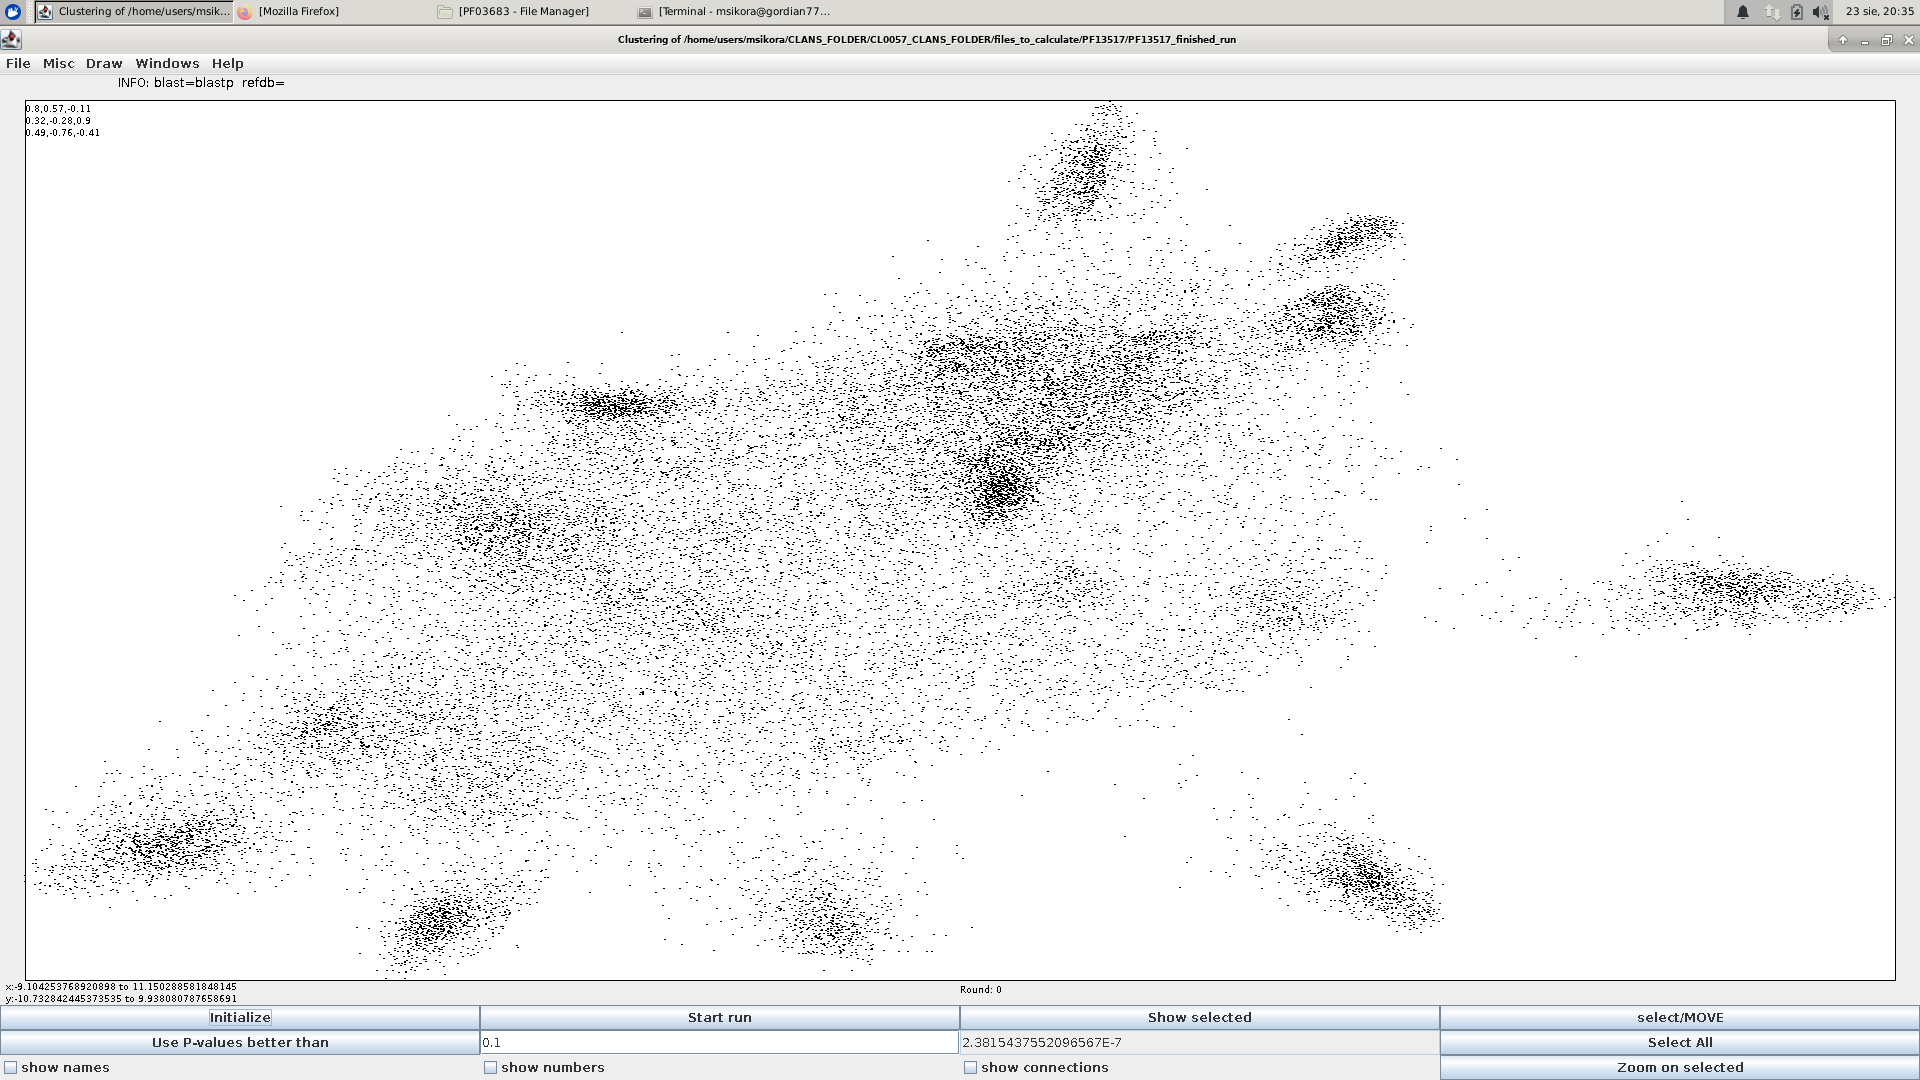
\includegraphics[width=0.5\textwidth]{PF13517_CLANS_1.png}
\end{center}
\end{figure}

\begin{figure}[H]
\begin{center}
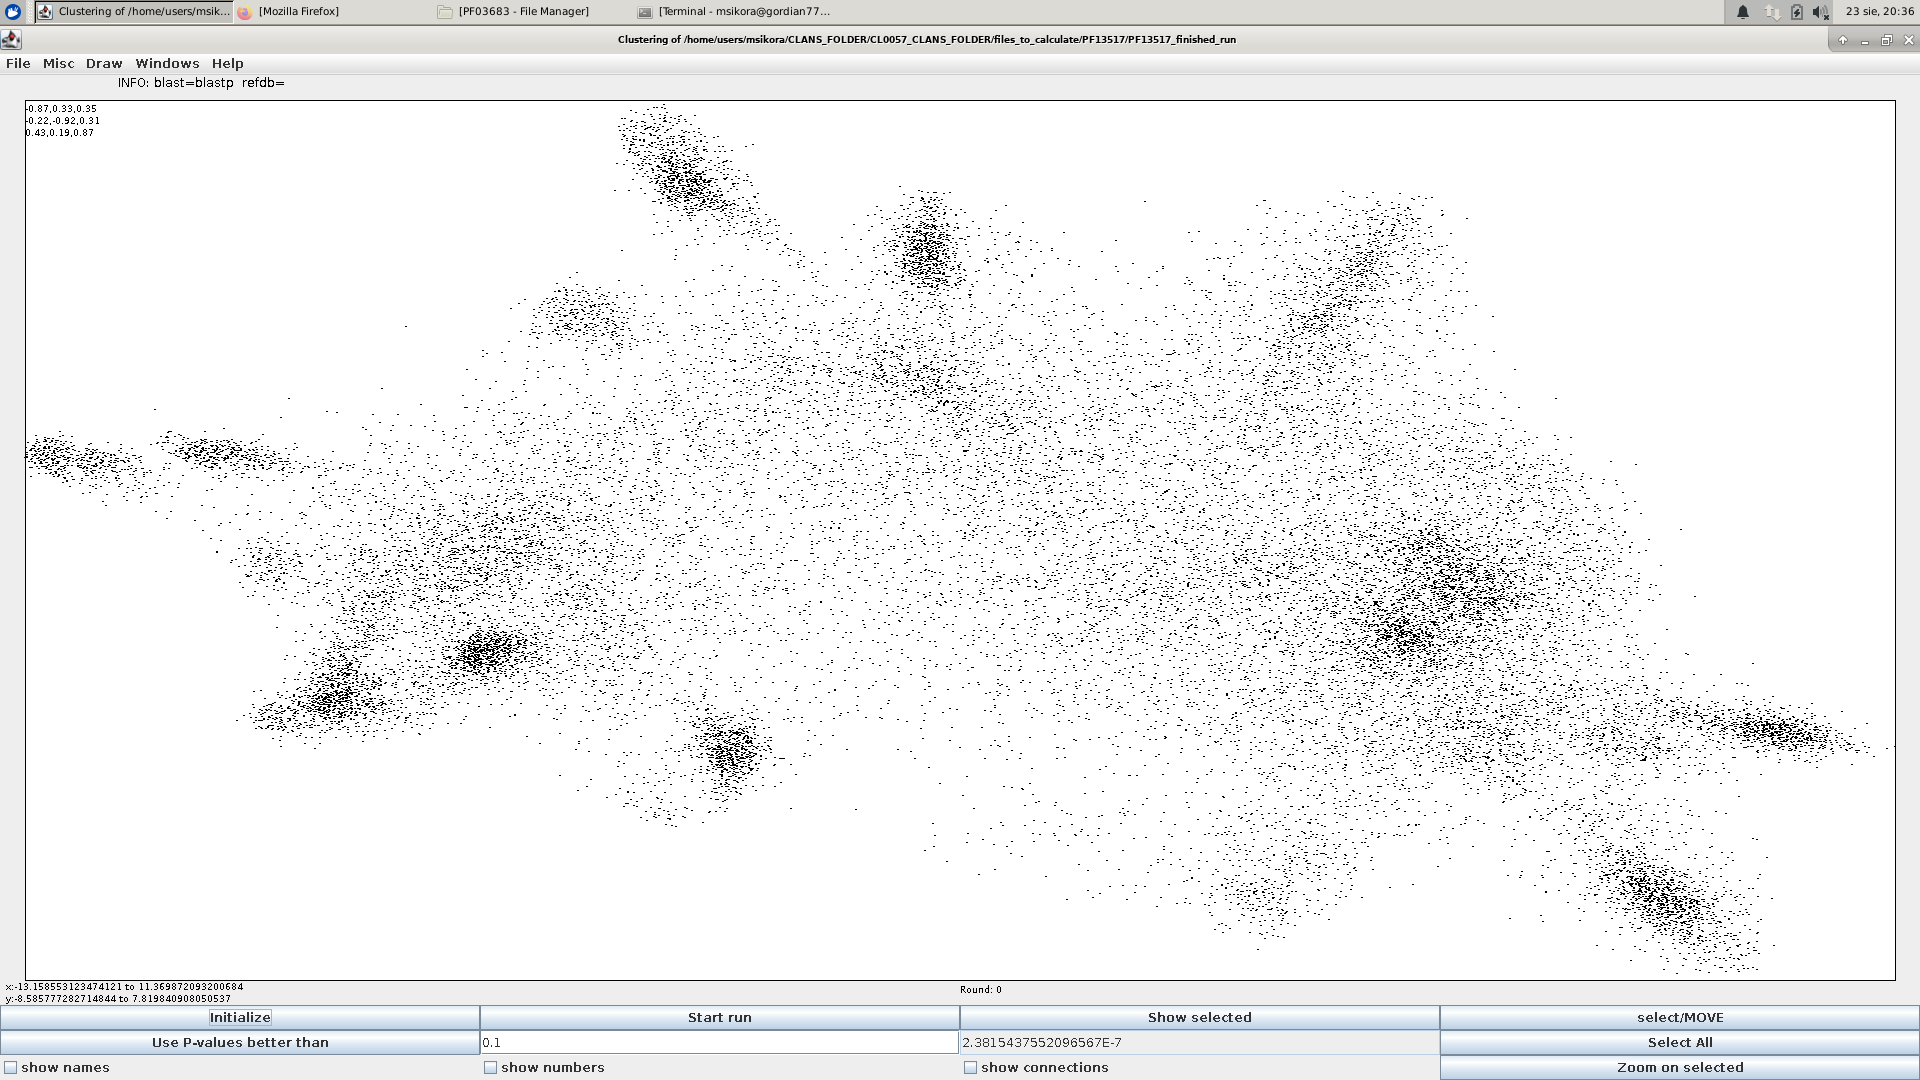
\includegraphics[width=0.5\textwidth]{PF13517_CLANS_2.png}
\end{center}
\end{figure}

   \subsubsection{PF05792 - Candida\_ALS / Candida agglutin-like (ALS) - No clan}
\begin{itemize}
    \item CLANS
\end{itemize}
Separating into 2/3 groups may be considered, but probably not necessary.

\begin{figure}[H]
\begin{center}
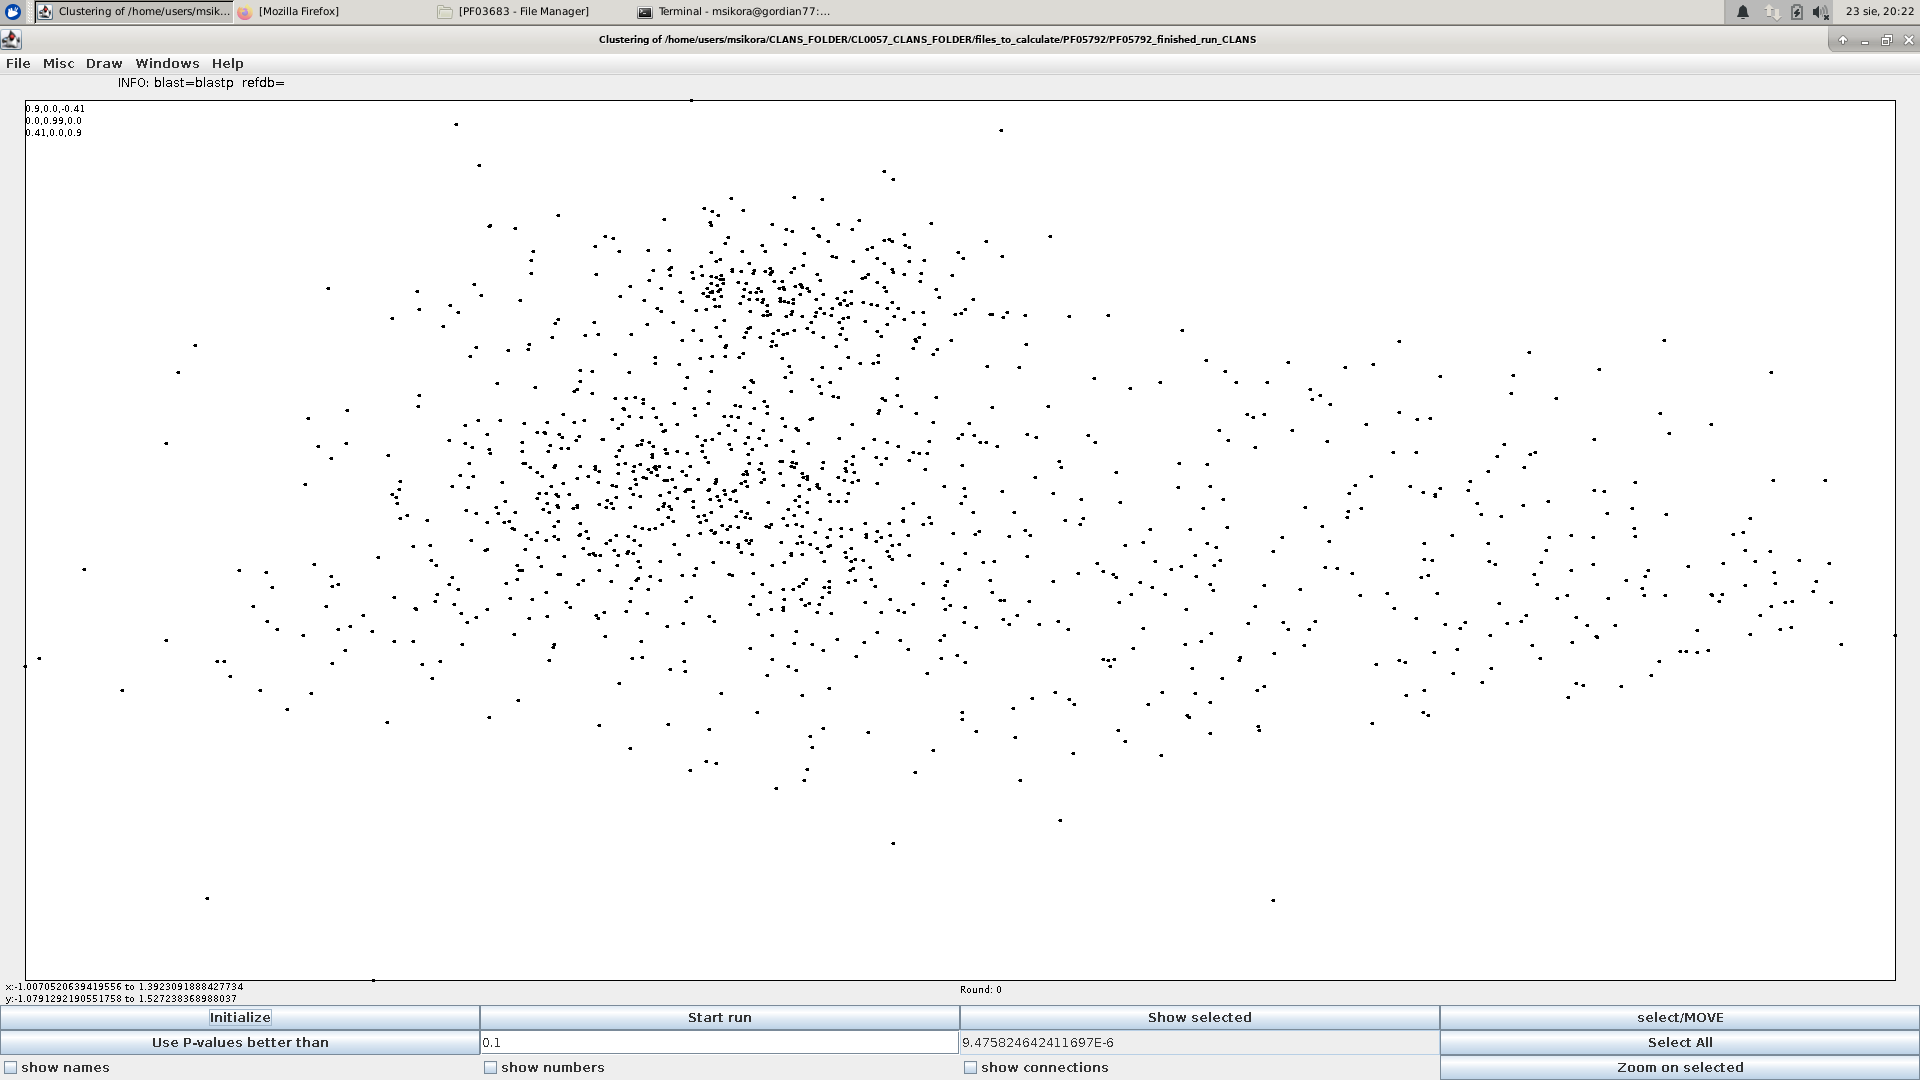
\includegraphics[width=0.5\textwidth]{PF05792_CLANS.png}
\end{center}
\end{figure}
